% !TEX root = Tesi.tex
\chead{}
\chapter{Our approach to modeling}

After summarily describing three different streams of real usage data obtained both from the physical and the virtual world in the last chapter, we now focus on expanding those representations in a more detailed way with the help of the Model Driven Engineering techniques briefly described in \ref{model-driven-techniques}. 
Concretely, the first two section objectives are to illustrate the defining languages (metamodels) for both the real usage data and the eCommerce platform interactions used in the previous examples and generate actual models based upon them representing the very same information.
Finally, in the last section of this chapter, we will be using the very same generation for updating the previously instantiated models leveraging model transformation techniques based upon usage pattern detection resulting from the Big Data analysis.

\section{Representing Real Usage Data}

\subsection{Metamodel}

The representation of the real usage data starts from the definition of the metamodel which defines the languages and processes from which to form a model without making statements about its content. In fact, a metamodel is itself a model that is used to describe another model using a modeling language and at a different level of abstraction.  

The figure in \ref{fig:real-usage-data-metamodel-diagram} describes the processed metamodel as a UML Class Diagram accordingly to the data retrieved for our real usage data analysis.

\vspace{0.5cm}
\begin{figure}[H]
  \centering
    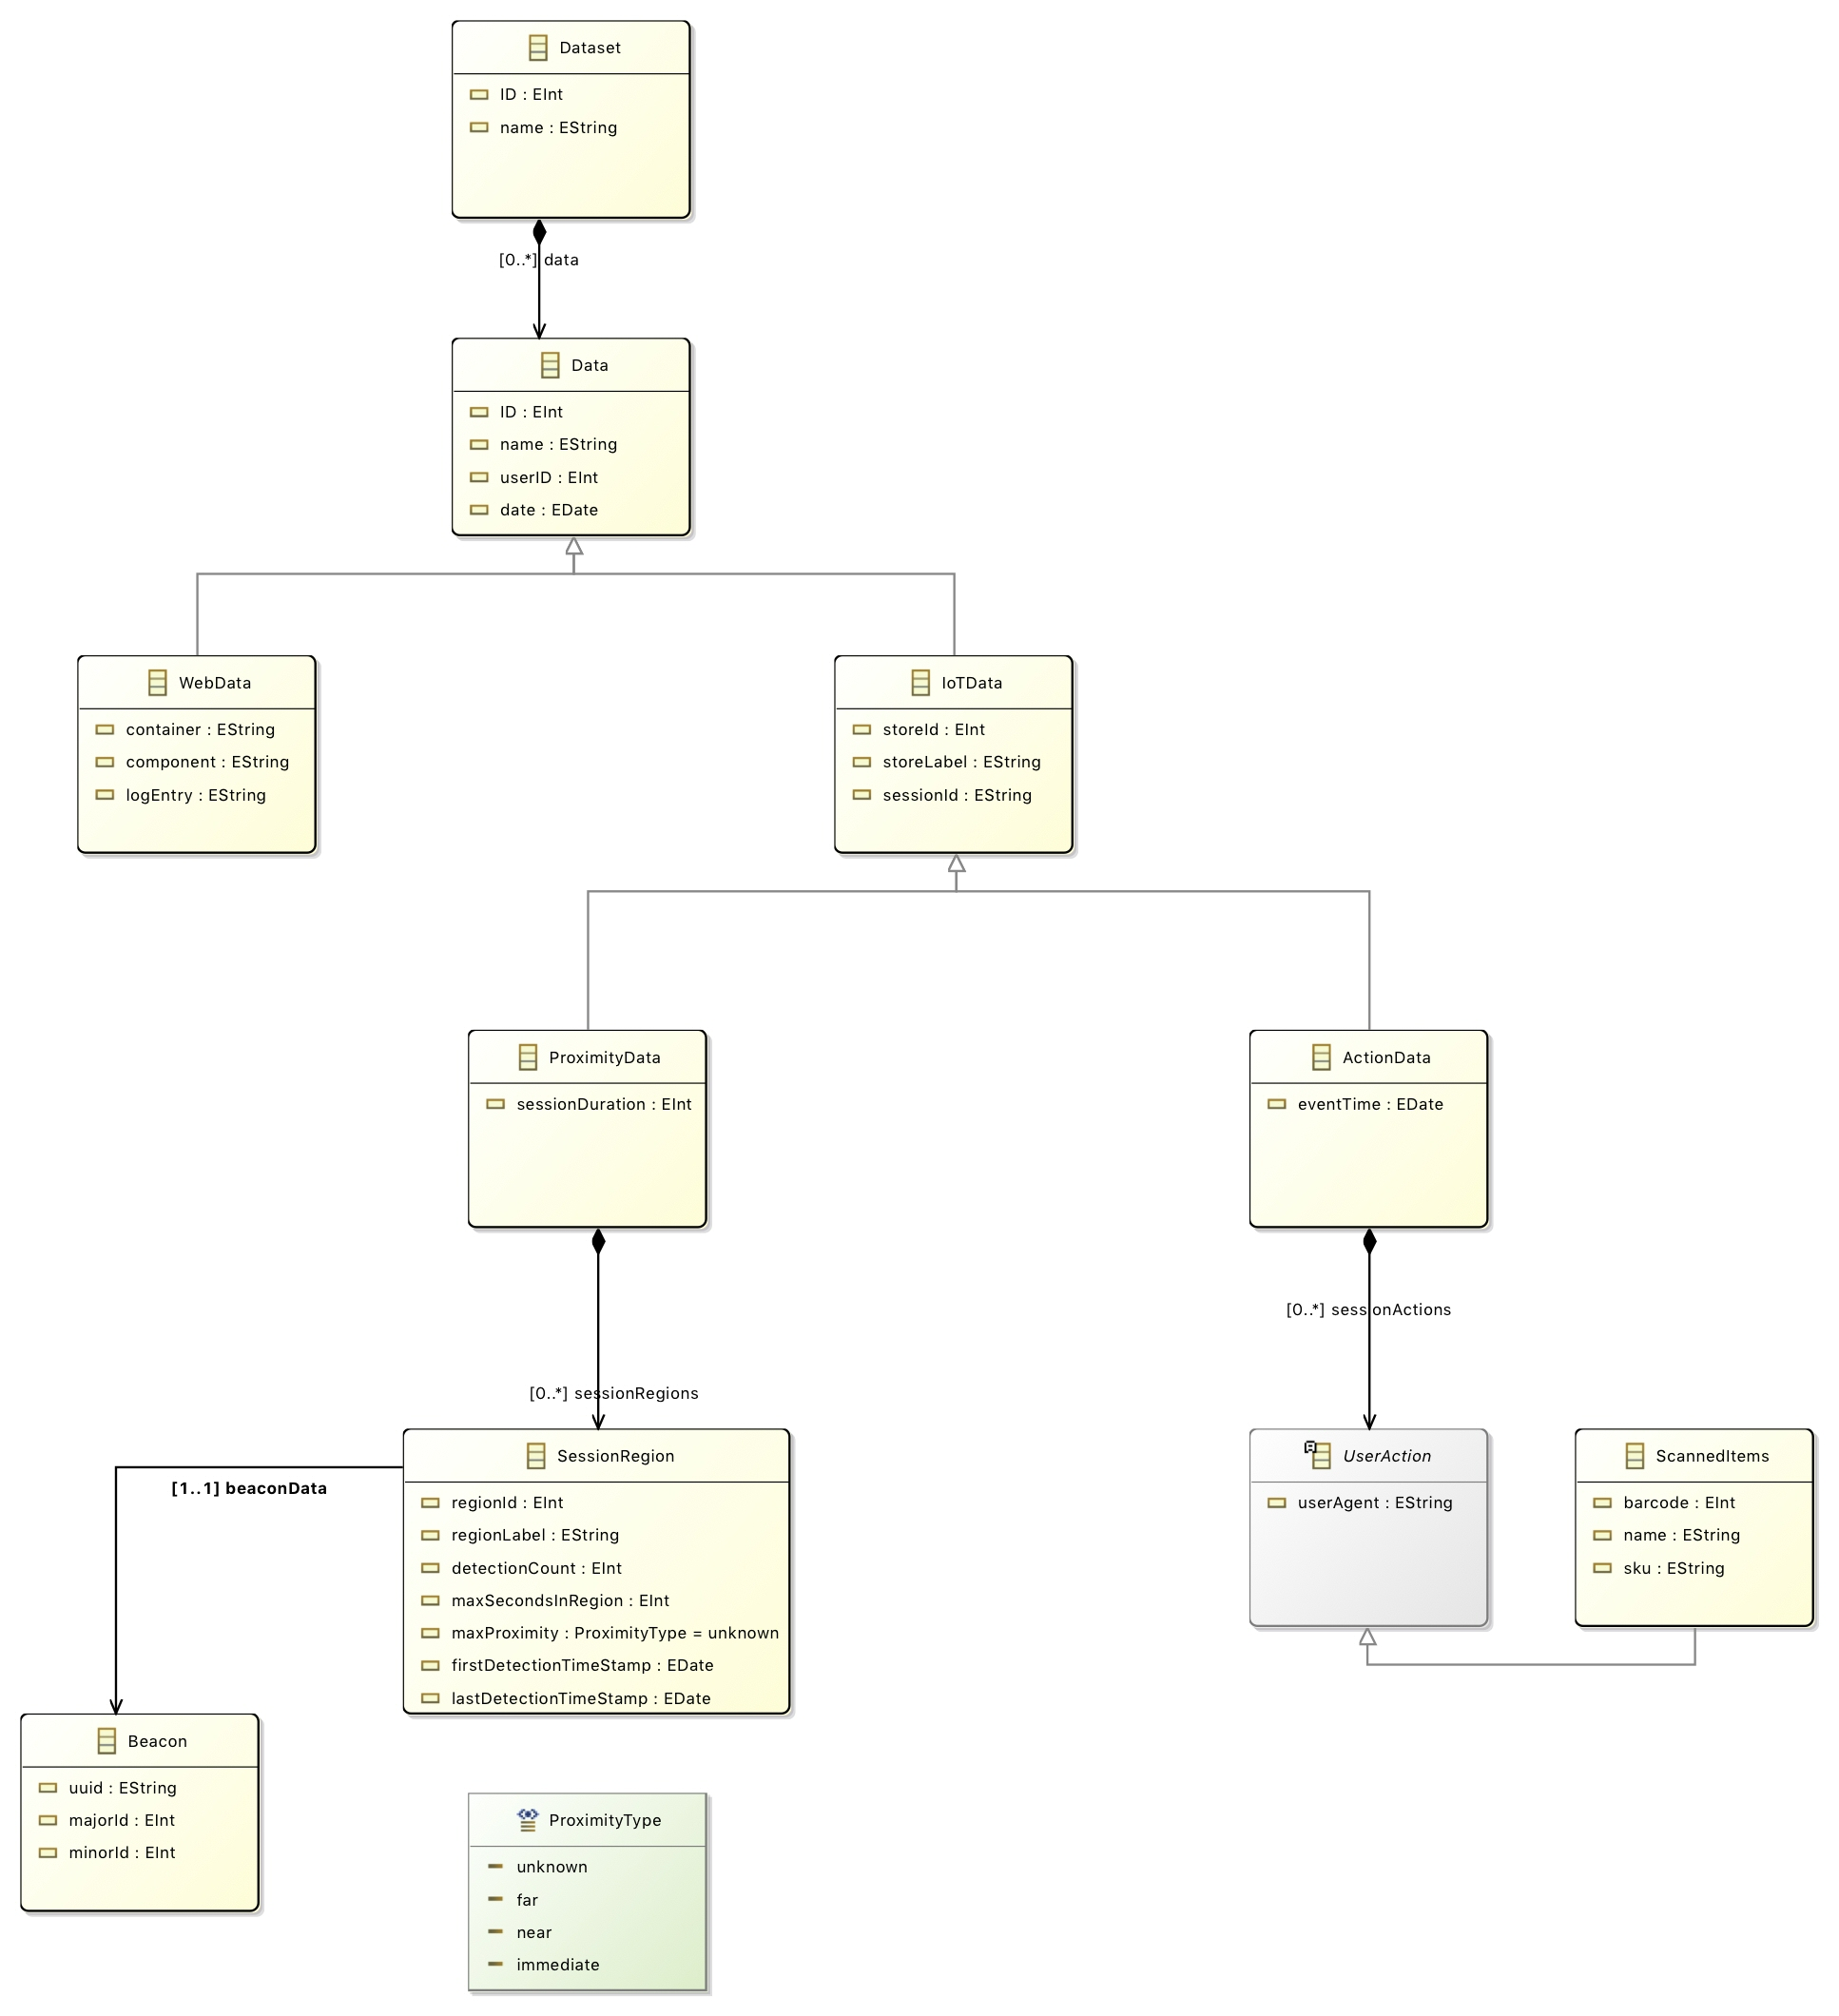
\includegraphics[height=19cm]{images/diagrams/RealUsageDataMetamodel.jpg}
  \caption{Real Usage Data Metamodel Diagram Class}
  \label{fig:real-usage-data-metamodel-diagram}
\end{figure}
\vspace{0.5cm}

\newpage
\subsection{Model}
\label{real-usage-data-model}
The RealUsageData metamodel defined above allow us to create dynamic instances which precisely map the real usage data collected from the web mining process and the IoT devices tracking. Figure \ref{fig:real-usage-data-model} illustrates this processed model in its eCore representation form in Eclipse and it is followed by the corrisponding XMI file content.

\vspace{0.5cm}
\begin{figure}[H]
  \centering
    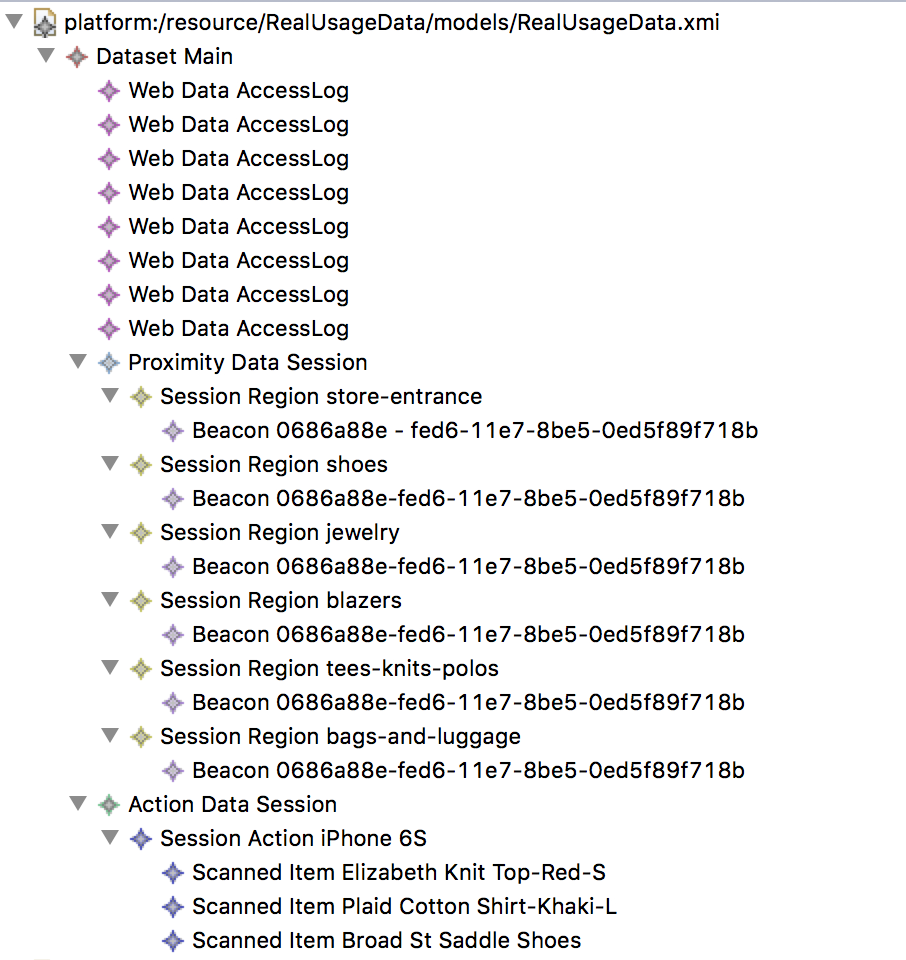
\includegraphics[height=12cm]{images/diagrams/RealUsageDataModel.png}
  \caption{Real Usage Data Model}
  \label{fig:real-usage-data-model}
\end{figure}
\vspace{0.5cm}

\lstset{language=XML}
\begin{lstlisting} 
<?xml version="1.0" encoding="UTF-8"?>
<RealUsageData:Dataset
    xmi:version="2.0"
    xmlns:xmi="http://www.omg.org/XMI"
    xmlns:xsi="http://www.w3.org/2001/XMLSchema-instance"
    xmlns:RealUsageData="RealUsageData"
    xsi:schemaLocation="RealUsageData ../metamodels/RealUsageData.ecore"
    ID="1" name="Main">
  <data xsi:type="RealUsageData:WebData"
      ID="1"
      name="AccessLog"
      userID="3045678"
      date="2017-11-29T17:06:49.000+0100"
      viewContainer="Homepage"
      viewComponent="TopMenu"
      eventType="click"
      parameterBindingGroup="Category/5"
      logEntry="GET /men.html / 200 0 - 29505"/>
  <data xsi:type="RealUsageData:WebData"
      ID="2"
      name="AccessLog"
      userID="3045678"
      date="2017-11-29T17:07:04.000+0100"
      viewContainer="Category #5"
      viewComponent="CategoryList"
      eventType="click"
      parameterBindingGroup="Category/15"
      logEntry="GET /men/shirts.html 200 0 - 29505"/>
  <data xsi:type="RealUsageData:WebData"
      ID="3"
      name="AccessLog"
      userID="3045678"
      date="2017-11-29T07:08:40.000+0100"
      viewContainer="Category #15"
      viewComponent="ProductList"
      eventType="click"
      parameterBindingGroup="Product/404"
      logEntry="GET /men/shirts/plaid-cotton-shirt-476.html 200 0 - 29505"/>
  <data xsi:type="RealUsageData:WebData"
      ID="4"
      name="AccessLog"
      userID="3045678"
      date="2017-12-04T06:37:15.000+0100"
      viewContainer="Product #404"
      viewComponent="RelatedProductList"
      eventType="click"
      parameterBindingGroup="Product/413"
      logEntry="GET /core-striped-sport-shirt-551.html 200 0 - 29505"/>
  <data xsi:type="RealUsageData:WebData"
      ID="5"
      name="AccessLog"
      userID="3045678"
      date="2017-12-04T06:37:21.000+0100"
      viewContainer=""
      viewComponent=""
      eventType="backButton"
      parameterBindingGroup=""
      logEntry="GET /men/shirts/plaid-cotton-shirt-476.html 200 0 - 29505"/>
  <data xsi:type="RealUsageData:WebData"
      ID="6"
      name="AccessLog"
      userID="3045678"
      date="2017-12-04T06:38:06.000+0100"
      viewContainer="Product #404"
      viewComponent="TopMenu"
      eventType="click"
      parameterBindingGroup="Category/16"
      logEntry="GET /men/tees-knits-and-polos.html 200 0 - 29505"/>
  <data xsi:type="RealUsageData:WebData"
      ID="7"
      name="AccessLog"
      userID="3045678"
      date="2017-12-04T06:38:20.000+0100"
      viewContainer="Category #16"
      viewComponent="TopSearch"
      eventType="submit"
      parameterBindingGroup="SearchText/blazer"
      logEntry="GET /catalogsearch/result/?q=blazer 200 0 - 29505"/>
  <data xsi:type="RealUsageData:WebData"
      ID="8"
      name="AccessLog"
      userID="3045678"
      date="2017-12-04T06:38:20.000+0100"
      viewContainer="Search Results"
      viewComponent="ProductList"
      eventType="click"
      parameterBindingGroup="Product/407"
      logEntry="GET /stretch-cotton-blazer-587.html 200 0 - 29505"/>
  <data xsi:type="RealUsageData:ProximityData"
      ID="9"
      name="Session"
      userID="3045678"
      date="2018-02-21T18:16:07.000+0100"
      storeId="8784"
      storeLabel="Madison1"
      sessionId="89376f84-065b -11e8- ba89-0ed5f89f718b"
      sessionDuration="345">
    <sessionRegions
        regionId="156"
        regionLabel="store-entrance"
        detectionCount="2"
        maxSecondsInRegion="5"
        firstDetectionTimeStamp="2018-02-21T18:09:07.000+0100"
        lastDetectionTimeStamp="2018-02-21T18:16:02.000+0100">
      <beaconData
          uuid="0686a88e - fed6-11e7-8be5-0ed5f89f718b"
          majorId="2553"
          minorId="79"/>
    </sessionRegions>
    <sessionRegions
        regionId="645"
        regionLabel="shoes"
        detectionCount="1"
        maxSecondsInRegion="24"
        maxProximity="near"
        firstDetectionTimeStamp="2018-02-21T18:09:20.000+0100"
        lastDetectionTimeStamp="2018-02-21T18:09:20.000+0100">
      <beaconData
          uuid="0686a88e-fed6-11e7-8be5-0ed5f89f718b"
          majorId="19029"
          minorId="49"/>
    </sessionRegions>
    <sessionRegions
        regionId="6875"
        regionLabel="jewelry"
        detectionCount="1"
        maxSecondsInRegion="15"
        maxProximity="far"
        firstDetectionTimeStamp="2018-02-21T18:10:15.000+0100"
        lastDetectionTimeStamp="2018-02-21T18:10:15.000+0100">
      <beaconData
          uuid="0686a88e-fed6-11e7-8be5-0ed5f89f718b"
          majorId="38415"
          minorId="59"/>
    </sessionRegions>
    <sessionRegions
        regionId="2563"
        regionLabel="blazers"
        detectionCount="1"
        maxSecondsInRegion="195"
        maxProximity="immediate"
        firstDetectionTimeStamp="2018-02-21T18:11:01.000+0100"
        lastDetectionTimeStamp="2018-02-21T18:11:01.000+0100">
      <beaconData
          uuid="0686a88e-fed6-11e7-8be5-0ed5f89f718b"
          majorId="25911"
          minorId="27"/>
    </sessionRegions>
    <sessionRegions
        regionId="456"
        regionLabel="tees-knits-polos"
        detectionCount="1"
        maxSecondsInRegion="10"
        maxProximity="immediate"
        firstDetectionTimeStamp="2018-02-21T18:14:56.000+0100"
        lastDetectionTimeStamp="2018-02-21T18:14:56.000+0100">
      <beaconData
          uuid="0686a88e-fed6-11e7-8be5-0ed5f89f718b"
          majorId="42037"
          minorId="36"/>
    </sessionRegions>
    <sessionRegions
        regionId="998"
        regionLabel="bags-and-luggage"
        detectionCount="1"
        maxSecondsInRegion="7"
        maxProximity="far"
        firstDetectionTimeStamp="2018-02-21T18:15:12.000+0100"
        lastDetectionTimeStamp="2018-02-21T18:15:12.000+0100">
      <beaconData
          uuid="0686a88e-fed6-11e7-8be5-0ed5f89f718b"
          majorId="37931"
          minorId="85"/>
    </sessionRegions>
  </data>
  <data xsi:type="RealUsageData:ActionData"
      ID="10"
      name="Session"
      userID="3045678"
      date="2018-02-22T15:27:09.000+0100"
      storeId="8784"
      storeLabel="Madison1"
      sessionId="89376f84-065b-11e8-ba89-0ed5f89f718b"
      sessionDuration="456">
    <sessionActions
        userAgent="iPhone 6S">
      <scannedItems
          barcode="042100005264"
          name="Elizabeth Knit Top-Red-S"
          sku="wbk012c-Red-S"/>
      <scannedItems
          barcode="042100005931"
          name="Plaid Cotton Shirt-Khaki-L"
          sku="msj006c-Khaki-L"/>
      <scannedItems
          barcode="042100007717"
          name="Broad St Saddle Shoes"
          sku="shm00110"/>
    </sessionActions>
  </data>
</RealUsageData:Dataset>
\end{lstlisting}

\section{Representing our eCommerce application with IFML}

As per briefly introduced in \ref{the-ifml-language}, interaction flow models are platform independent-level models which can be used to define the interactions between the users of an application and the application itself. They describe the user interface components required at the front-end of the
application, without specifying layout details of these elements enhancing the separation of concerns among developers and UX designers where the latter build the user interface accordingly to an interaction flow model. Besides defining components of the User Interface, the interaction flow model explains how data flows among different sections of the application upon triggering events and introduces the business logic carried out using this data.

\subsection{IFML Metamodel}

The IFML metamodel is organized into three packages: the Core package, the Extension package and the DataTypes package. The Core package contains the concepts that build up the interaction infrastructure of the language concerning InteractionFlowElements, InteractionFlows and Parameters. The Extension package extends the Core package components with more complex behaviors. The DataTypes package contains the custom data types defined by IFML.

By using the primitive data types from the UML metamodel and a UML representation for the IFML Domain Model, the IFML metamodel specifies a set of UML metaclasses as the foundation for the IFML metaclasses.

The following is the structure of the high-level representation of the IFML metamodel and its areas of concern:

\begin{itemize}
  \item IFML Model
  \item Interaction Flow Model
  \item Interaction Flow Elements
  \item View Elements
  \item Events
  \item Specific Events and View Components
  \item Parameters
  \item Expressions
  \item ContentBinding
\end{itemize}

Figure \ref{fig:simple-ifml-core-model} shows an excerpt of the IFML metamodel. As can be seen, IFMLModel is the top-level container of all the model elements and represents an IFML model. It contains an InteractionFlowModel which is the user view of an application, a DomainModel represented in UML and optionally ViewPoints. The concepts extending ViewContainer, ViewComponets, ViewComponentPart, and ViewElementEvent represent the visual elements of an IFML model.

\vspace{0.5cm}
\begin{figure}[H]
  \centering
    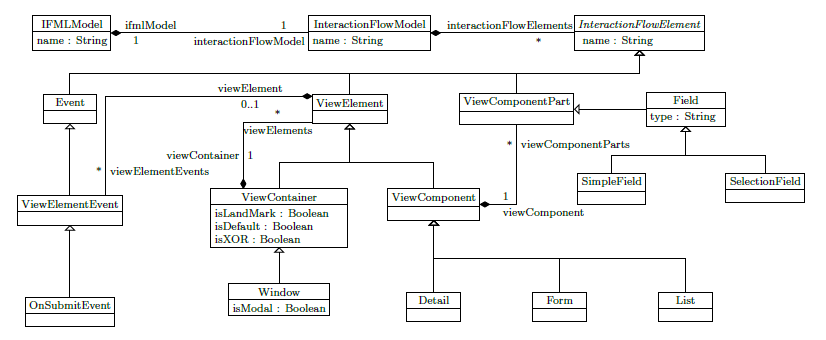
\includegraphics[width=12cm]{images/diagrams/ifml-metamodel.png}
  \caption{Simple Ecore model of an IFML subset.}
  \label{fig:simple-ifml-core-model}
\end{figure}
\vspace{0.5cm}

\subsection{Model}

As per mentioned in the last subsection, interaction flow models are described using the Interaction Flow Modelling Language and, together with the domain model and optionally viewpoints, they form the core of the IFML model.

Essentially, the domain model objective is offering to the interaction flow references about the content available. An example of a domain model for an e-commerce website is given in figure \ref{fig:domain-model-uml-ecommerce}   

\vspace{0.5cm}
\begin{figure}[H]
  \centering
    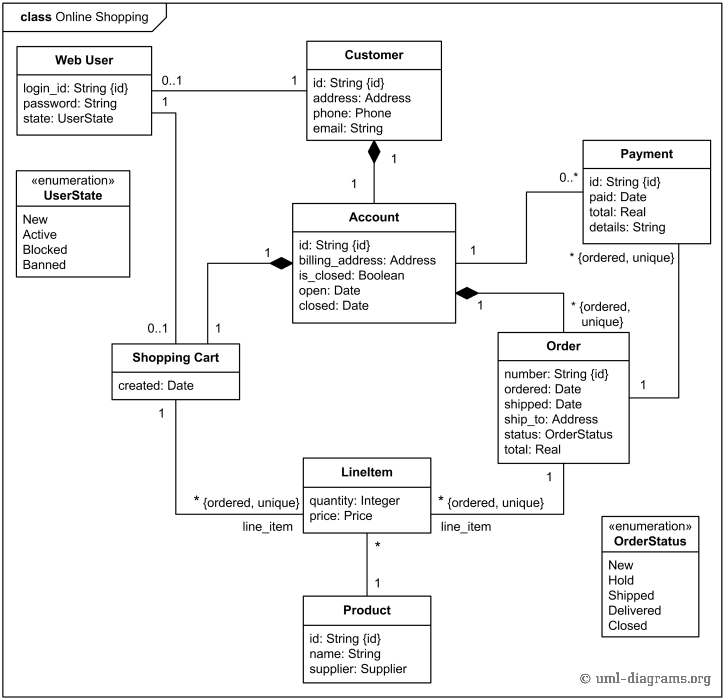
\includegraphics[width=12cm]{images/diagrams/domain-model-uml-ecommerce.png}
  \caption{Domain Model UML Class Diagram ecommerce example.}
  \label{fig:domain-model-uml-ecommerce}
\end{figure}
\vspace{0.5cm}

Although some partial IFML model representations for the Madison Island eCommerce platform have been already summarily introduced in \ref{navigational-modeling-for-the-web}, in this subsection we examine them in more detail and with a more global approach not strictly related to the navigational modeling. The final goal is to model, taking advantage of the IFML metamodel described just above, an IFML model which would represent the main pages and interactions of the website on top of which we would perform transformations dictated by the Real Usage Data models illustrated in \ref{real-usage-data-model}

\section{Updating the web models through real usage data}

\subsection{Transformation}

\subsection{Updated Models}
